\documentclass[]{article}

\usepackage{amsmath,amssymb}
\usepackage{bbm}
\usepackage{xcolor}
\usepackage{graphicx}
\graphicspath{ {./figs/} }
\usepackage{hyperref}

\newcommand{\argmax}[1]{\text{arg}\hspace{-2pt}\max\limits_{#1}}
\newcommand{\bvec}[1]{\boldsymbol{#1}}
\newcommand{\assumption}[1]{{\color{red}#1}} 
\usepackage{listings}
\newcommand{\codeword}[1]{\texttt{\textcolor{blue}{\lstinline{#1}}}
}

\author{C. C. Chang, C. C. Chen, C. K\"orber, T. Humble, J. Ostrowski}

%opening
\title{Notes}

\begin{document}

\maketitle

\section{Main Idea}

Integer linear programming is pretty useful apparently. The problem boils down to solving a system of linear equations and inequalities. Just Google linear integer programming, and Wikipedia has a good example for the general type of problem that is being solved. The underlying problem is classically NP-hard, so there is an possibility to exponentially speed-up this entire set of problems with quantum annealing. The main idea here is to encode inequalities into a quantum annealer.

Quick overview, a quantum annealers solves a QUBO problem (which is basically Ising Model). The problem can be boiled down to the form $x Q x$ where $x$ is a vector of qubits (so they can only take values of 0 or 1 or some super-position). We have to ``program'' $Q$ to solve our problem.

Following https://arxiv.org/abs/1812.06917 we know 1) how to encode fixed-precision numbers into a set of qubits. 2) We also know how to encode higher order problems (\textit{e.g.} $J x^4 + Q x^2$). 3)  We also learned that in general, since QA can only solve for the global minimum, we must optimize the squared-residual of a set of equations / inequalities. Anyways, read the paper if you haven't already.

To encode an inequality of the form $A < y < B$ we can introduce an auxiliary qubit $y_a$ such that the logical qubit is $Y = (y, y_a)$ (where $y$ and $y_a$ are logical qubits representing fixed-precision numbers encoded by $n$ qubits). The inequality is then encoded as minimizing the following $C_1 Y^4 - C_2 Y^2 + C_3$ such that we get a mexican-hat potential. Basically this was inspired from spontaneous symmetry breaking. I'm sure this can be connected to solving scalar phi-4 theory if we reallllly want to go there. But tuning the $C$s will tune the radius of the degeneracy and therefore change the range of $A$ and $B$.  Also $C_3$ shifts the minimum to zero, which is useful if we want to keep the energy positive, and interpret it as the squared-residual. Travis suggested that this might be connected to ``slack variables'' (see https://arxiv.org/abs/1811.11538 that I haven't read yet).

I'm worried that $y_a$ has nonlinear dependence with $y$ as we walk along the degeneracy though, which in practice may be an issue. Though increasing the number of qubits used to represent a fixed-precision decimal solves this problem exponentially quickly.

\section{Implementation}

So I have been following up on @CCChen's notes and extended the software a bit.
The software is a Python module which converts a set of inequalities to the matrix we want to have on the quantum computer.
I was wondering about the details of the derivation and if there are assumptions which may have consequences for the parameter space.
Assumptions are defined by constraints which potentially make our approach not true given only \eqref{max-x} and \eqref{condition-x}.
I have highlighted assumptions with the \assumption{green text}.

A little bit different to @CCChen's, I have introduced a matrix $Q$ which maps bit vectors to integer vectors.
This helps the software a bit to stay general---and me to mimic the physics I am used to.

Let me know if you have any questions.

\subsection{Integer problem optimization}
What we eventually want to solve a maximization problem
\begin{equation}\label{max-x}
	\vec x_0 = \argmax{\vec x} \left( \vec c \cdot \vec x\right) \, ,
\end{equation}
where $\vec x_0$ is the $\vec x$ which maximizes the above gradient under a set of inequalities
\begin{align}\label{condition-x}
	A \vec x - \vec b &\leq \vec 0 \, , &
	A &\in \text{Mat}(\mathbbm R, (N_x, N_e)) \, , &
	\vec b &\in \mathbbm{R}^{N_e} \, &
	\vec c &\in \mathbbm{R}^{N_x} \, , &
	\vec x &\in \mathbbm{N}^{N_x}\, .
\end{align}
In this definition, the set of natural numbers $\mathbbm{N}$ includes zero (but no negative numbers).
The additional dimension $N_e$ is the number of inequalities we have.

In principle, one could also have inequalities of the form $A_{ij} x_j - b_j \geq 0$ or any other relations.
But equation \eqref{condition-x} completely sufficient to characterize all problems with, because, for example a $\geq$ in a certain row can be obtained by multiplying the row with $-1$ and a $<$ can be obtained by an infinitesimal shift in $\vec b$.
Equalities are a little bit different, in principle they can be brought to this form by combining $A_{ij} x_j - b_j \geq 0$ with $A_{ij} x_j - b_j \leq 0$, but this introduces two constraints.

When introducing the slack variable, we can summarize the constraints in a single equation
\begin{align}\label{slack-optimization}
	\vec x_0 &= \argmax{\vec x} \left( \vec c \cdot \vec x - p f(\vec x) \right) \, , \\
	f(\vec x) &= \min\limits_{\vec s}\left[
		\left(\tilde A \vec x - \vec{\tilde{b}} + D \vec s\right) \cdot \left(\tilde A \vec x - \vec{\tilde{b}} + D \vec s\right)
	\right] \, , &
	p &\gg \max\limits_{\vec x}\left(\vec c \cdot \vec x\right) \, .
\end{align}
The quantities introduced in this equation are defined by
\begin{align}
	\vec s &\in \mathbbm{N}^{N_e} \, , \qquad
	D \in \text{Mat}(\{0, 1\}, (N_e, N_e)) \, .
\end{align}
More specifically $D$ is diagonal and it's entries are either one or zero (they are zero when we have an equality instead of an inequality).
The entries 
\begin{align}
	\tilde A = (10^{m} A) & \in \text{Mat}(\mathbbm Z, (N_x, N_e)) \, , &
	\vec{\tilde{b}} &= (10^m \vec{b}) \in \mathbbm{Z}^{N_e}
\end{align}
are rescaled with a factor $10^m$ such that all entries of $\tilde A_{ij}$ and $\tilde b_{i}$ are integer valued.
\assumption{This assumes that $A$ and $\vec b$ are given for finite precision.}

Note that \assumption{for this particular condition we need that $x$ is constrained} and in principle \assumption{$p > \max\limits_{\vec x}\left(\vec c \cdot \vec x\right)$} would be suffice.
However, this would require solving the problem.


\subsubsection{Proof}
Because $\tilde A$ and $\vec{\tilde{b}}$ are integer valued, one can find a vector $\vec s$, such that 
\begin{equation}
	\forall \vec x \quad \exists \vec s \in \mathbbm{N}^{N_e} \, : \, \tilde A \vec x - \vec{\tilde{b}} + D \vec s = 0 \, .
\end{equation}
Thus $f(\vec x) \geq 0$ and furthermore
\begin{equation}
	f(\vec x_s) = 0 \iff A \vec x - \vec{b} \leq \vec 0 \, .
\end{equation}
From $f(\vec x_s) = 0 \Rightarrow A \vec x - \vec{b} \leq \vec 0$ is true because each component of $\vec s$ is $\geq 0$ and thus $\tilde A \vec x - \vec{\tilde{b}} \leq \vec 0$.
This is invariant under scaling with $10^{-m}$.

Also, $A \vec x - \vec{b} \leq \vec 0 \Rightarrow f(\vec x_s) =  0  $ is true because if $A \vec x - \vec b \leq 0 \Rightarrow \tilde A \vec x - \vec{\tilde{b}} \leq \vec 0$.
And since $- \vec m = \tilde A \vec x - \vec{\tilde{b}} \leq \vec 0$ for a vector $\vec m \in \mathbbm{N}^{N_e}$, we can pick $\vec m = \vec s$.

Therefore, if $p$ is sufficiently large we know that the \eqref{slack-optimization} is maximal if $f(\vec x) = 0$ and the maximum of \eqref{slack-optimization} is thus equal to $\max\limits_{\vec x}(\vec c \cdot \vec x)$ under the specified constraints at the same location $\vec x_0$.


\subsection{Map to bits}
Next we want to code up $\vec x$ and $\vec s$ as bit vectors, e.g.,
\begin{equation}
	q = \sum_{n=0}^{N_b-1} 2^n \psi_n^{(q)} \, , \qquad \psi_n^{(q)} \in \{ 0, 1\}\, .
\end{equation}
Here, \assumption{the number of bits reduces the available number space to finite numbers}.
This could potentially mean, if $N_b$ for $\vec x$ is not large enough, we do not probe $\vec x _0$.
Also if the constrained space needs be extensively probed, e.g., if the optimal value $\vec x_0$ is far away from the boundary, we might need large $N_b$ to have large $\vec s$.
One may even think about having different numbers of bits for $\vec x$ and $\vec s$.

With this definition, we can introduce a new basis and map between integers and bits such that
\begin{align}
	q &= \vec Q \cdot \bvec{\psi}^{(q)} \, , &
	\bvec{\psi}^{(q)} &\in \{ 0, 1\}^{N_b} \,, &
	\vec Q^T &= \left(1, 2, 2^2, \cdots,  2^{N_b -1} \right) \, .
\end{align}

With these definition we have that
\begin{align}
	\vec \xi 
	&= 
	\begin{pmatrix}
		\vec x \\
		\vec s 
	\end{pmatrix}
	= Q \bvec \psi^{\left( \vec \xi \right)} \, , &
	Q 
	&=
	\begin{pmatrix}
		\vec Q^T & \vec 0^T & \vec 0^T & \cdots & \vec 0^T \\
		\vec 0^T & \vec Q^T & \vec 0^T & \cdots & \vec 0^T \\
		\vdots   & \ddots   & \ddots   & \ddots & \vdots \\
		\vec 0^T & \vec 0^T & \vec 0^T & \cdots & \vec Q^T
	\end{pmatrix}\, .
	\, , & 
	\psi^{\left( \vec \xi \right)} & \in \left(\{0, 1\}^{N_b}\right)^{N_e + N_x} \, ,
\end{align}
in other words $Q$ is a $(N_e + N_x) \times N_b(N_e + N_x)$ matrix.

To separate spaces, if introduced the notation that
\begin{itemize}
	\item greek vectors like $\vec \xi$ denote combined $\vec x$ and $\vec s$ space,
	\item specifically the greek letter $\psi = 0, 1$ denotes bits,
	\item the bold face vectors like $\bvec \psi^{\left( \vec \xi \right)}$ denote vectors in the bit basis (which do not necessarily have to be $0,1$).
\end{itemize}


\subsection{Integer problem optimization using bits}
Now we can map \eqref{slack-optimization} to the new basis
\begin{align}
	\vec x_0 
	&= \argmax{\vec x}\left(\max\limits_{\vec s}
	\left( \bvec \gamma \cdot \bvec \psi^{\left( \vec \xi \right)} - p \phi\left(\bvec \psi^{\left( \vec \xi \right)}\right)\right)\right) \, , &
	\bvec \gamma &= \begin{pmatrix}
		\vec c \\ \vec 0
	\end{pmatrix} \cdot Q \in \mathbbm{R}^{(N_x + N_e )N_b} \, , 
\end{align}
where I have pulled out the $\min$ over $\vec s$ (which becomes a $\max$ because of the minus sign) which is irrelevant for the $\bvec \gamma$ dot product since the $s$-component vanishes.
The constrained $f \mapsto \phi$ is now given by
\begin{align}\label{bit-penalty}
	\phi\left(\bvec \psi^{\left( \vec \xi \right)}\right)
	&=
	\left[
	\left(
		\tilde{\alpha} Q \bvec \psi^{\left( \vec \xi \right)} - \vec{\tilde{b}}\right) 
		\cdot \left({\tilde{\alpha}} Q \bvec \psi^{\left( \vec \xi \right)} - \vec{\tilde{b}}\right)\right]
	\, , \\
	{\tilde{\alpha}} &= \left(\tilde{A},  D \right) \in \text{Mat}(\mathbbm{Z}, (N_x + N_e, N_e))\, ,
\end{align}
where the above quantities are split up in $\vec x$ and $\vec s$ space.

In the following context we use that the components of the bit vector are either one or zero and thus $\psi^{\left( \vec \xi \right)}_\nu = \psi^{\left( \vec \xi \right)}_\nu \psi^{\left( \vec \xi \right)}_\nu$.
Also, to simplify notation, indices to bit-space vectors are given by $\mu, \nu$, indices to $(\vec x, \vec s)$-space vectors are given by $i, j, k$ and it is summed over repeated entries.
The argument of equation \eqref{bit-penalty} simplifies to
\begin{equation}
	\label{eq:constraint-matrix}
	\phi\left(\bvec \psi^{\left( \vec \xi \right)}\right)
	=
	\psi^{\left( \vec \xi \right)}_\nu
	\left[
		(\tilde \alpha Q)_{i\nu} (\tilde \alpha Q)_{i\mu}
		-  \delta_{\nu\mu}\tilde{b}_i (\tilde \alpha Q)_{i\mu}
		- \delta_{\nu\mu} (\tilde \alpha Q)_{i\nu} \tilde{b}_i
	\right]
	\psi^{\left( \vec \xi \right)}_\mu
	+ \tilde{b}_i \tilde{b}_i \, .
\end{equation}
Because the we compute the location of the optimal value, we can neglect the constant shift $\tilde{b}_i \tilde{b}_i$.
Furthermore, we can combine the search for optimal $\vec x$ and $\vec s$ by a search for optimal $\vec \xi$ and hence optional $\bvec \psi^{\left( \vec \xi \right)}$.
This results in
\begin{align}
	\bvec \psi^{\left( \vec \xi \right)}_{0} 
	&=
	\argmax{\psi^{\left( \vec \xi \right)}}\left( 
		\bvec \psi^{\left( \vec \xi \right)} \cdot \Omega \bvec \psi^{\left( \vec \xi \right)}
	\right)
	\, , \qquad
	\vec x_0 =  (\mathbbm 1, 0) Q \bvec \psi^{\left( \vec \xi \right)}_{0} 
	\\
	\Omega_{\nu\mu}
	&=
	\delta_{\nu\mu} \gamma_i Q_{i\nu}
	- p \tilde \alpha_{ij} Q_{j\nu} \tilde \alpha_{ik} Q_{k\mu}
	+ 2 p \delta_{\nu\mu}\tilde{b}_i \tilde \alpha_{ij} Q_{j\mu}
\end{align}

\section{Example}
In this section we present the optimization of
\begin{equation}
	\label{eq:g}
	g(x_0, x_1) = 8 -(x_0 - 2)^2 - (x_1 - 2)^2 \, ,
\end{equation}
under different constraints.

This repository contains the module \codeword{qlp} which provides functionality to implement the problem for bit operations.

\begin{figure}
	\centering
	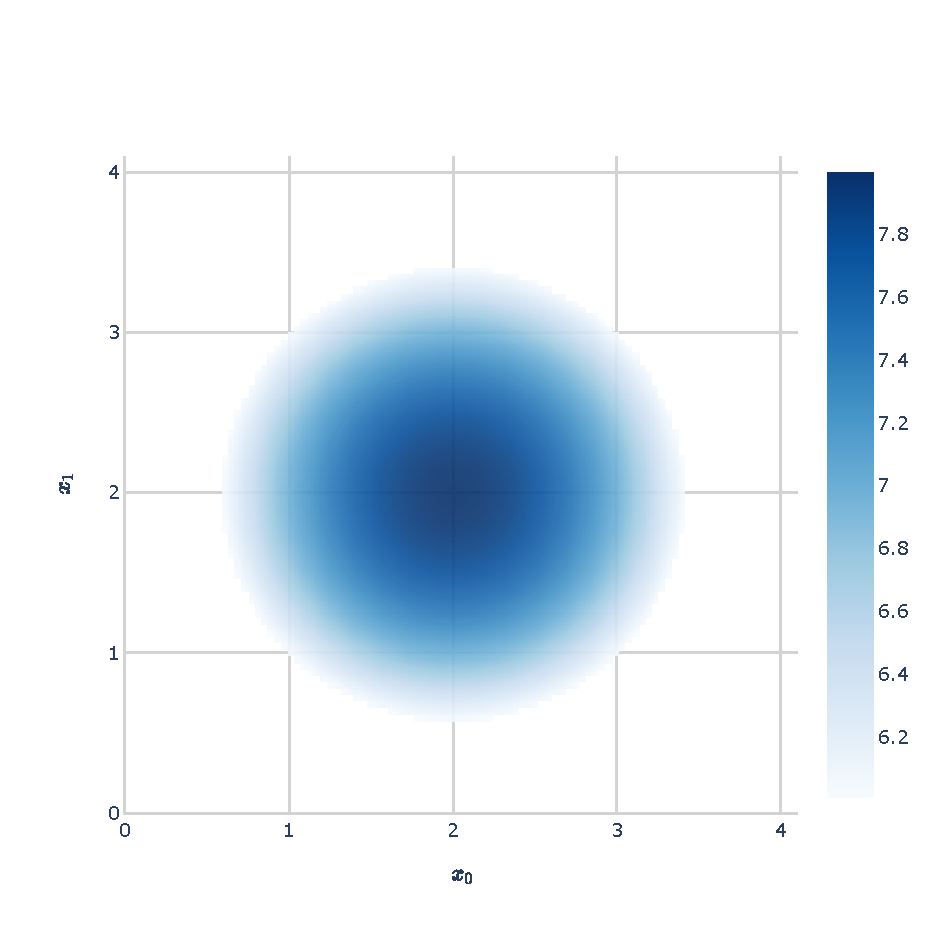
\includegraphics[width=0.5\textwidth]{contour-opt}
	\caption{
		\label{fig:g}
		Contour plot of $g$ defined in eq.~\eqref{eq:g}.
		Darker colors denote larger values, lighter colors denote smaller values.
		Values below $6$ are displayed as white.
	}
\end{figure}

In the bit basis, $g$ is implemented as
\begin{equation}
	M_{\alpha \beta}
        =
        - Q_{0\alpha}Q_{0\beta}
        - Q_{1\alpha}Q_{1\beta}
        + 4Q_{0\alpha}\delta_{\alpha\beta}
        + 4Q_{1\alpha}\delta_{\alpha\beta}
   \, , \qquad
   g(x_0, x_1) = \psi_\alpha M_{\alpha \beta} \psi_\beta + \vec b^2\, .
\end{equation}
This matrix is obtained by running \codeword{qlp.example.get_omega_0}.

We implement the following three constraints (see also fig. \ref{fig:constraints})
\begin{equation}
	\label{eq:constrained}
	0
	\leq
	f(\vec x)
	=
	\begin{cases}
		4 - x_0 - x_1 & (A) \\ 
		6 - x_0 - 3 x_1 & (B) \\
		3 - x_0 - x_1 & (C)
	\end{cases}
	\, .
\end{equation}

\begin{figure}
	\centering
	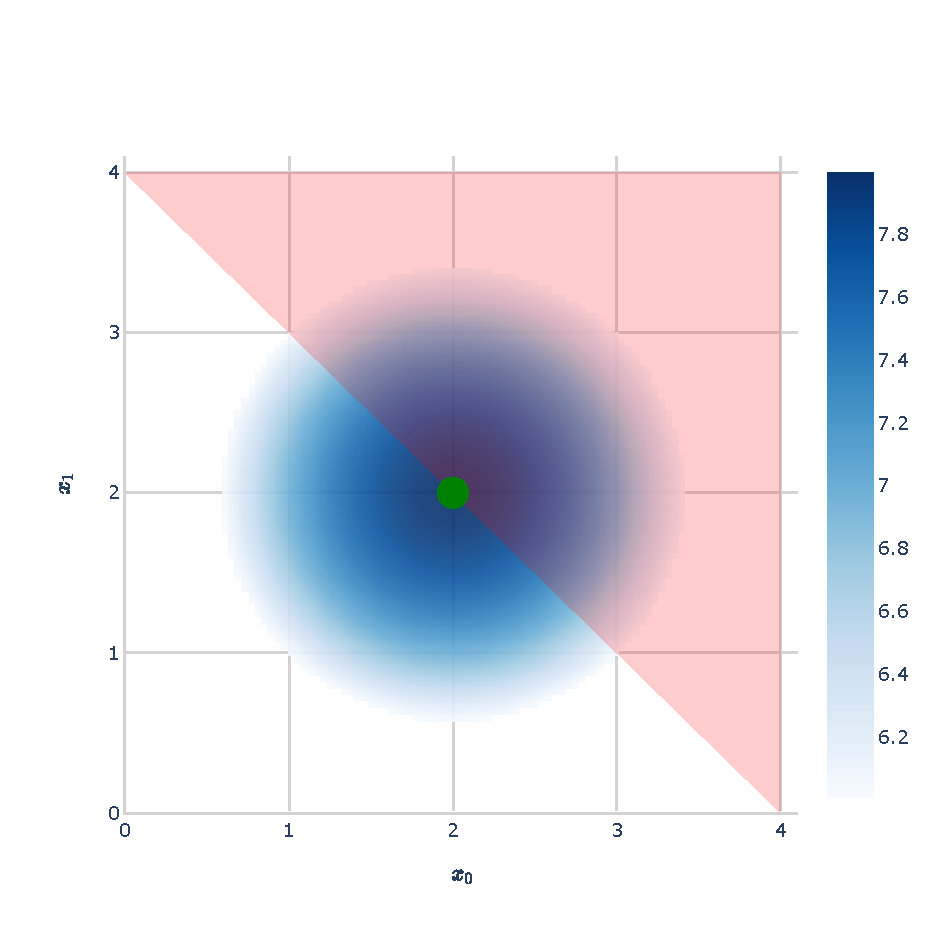
\includegraphics[width=0.32\textwidth]{contour-constraint-1}
	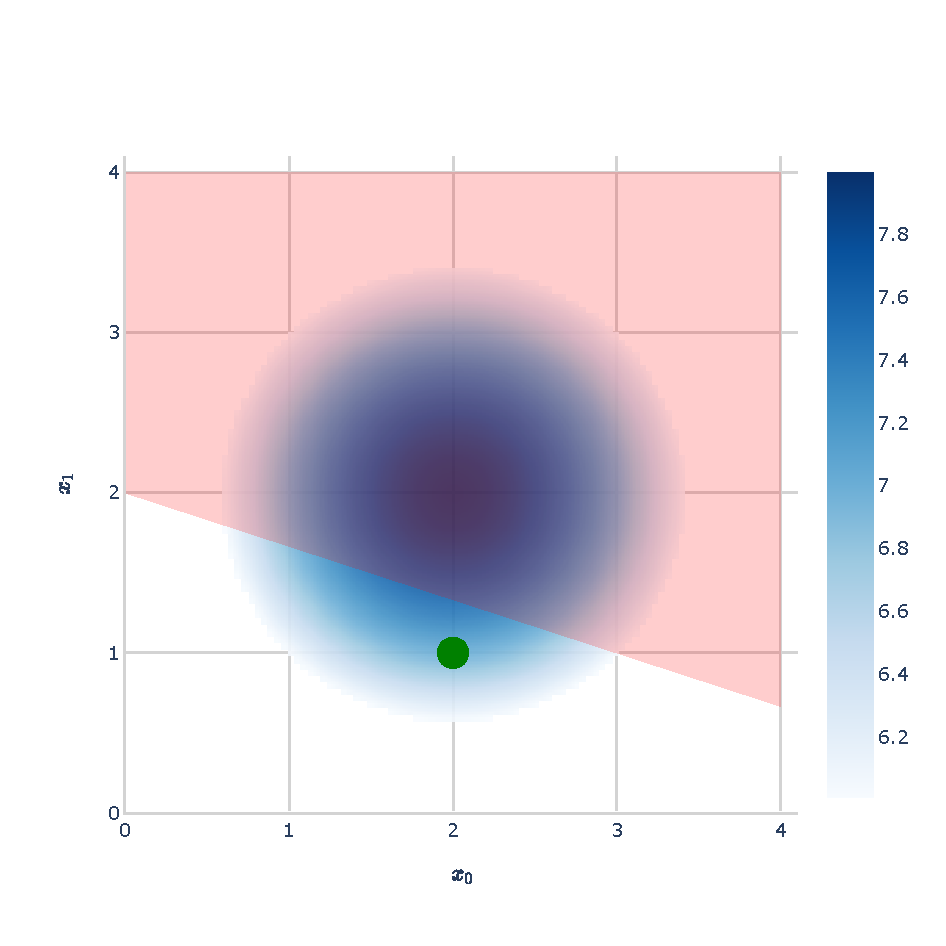
\includegraphics[width=0.32\textwidth]{contour-constraint-2}
	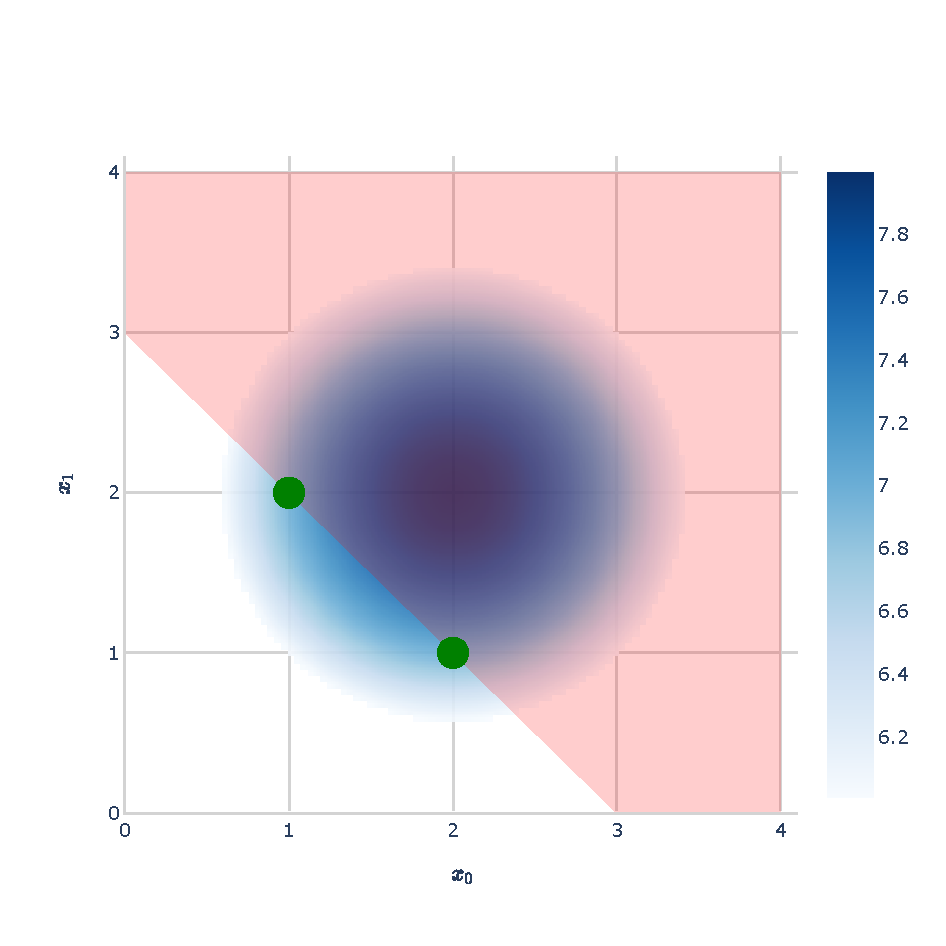
\includegraphics[width=0.32\textwidth]{contour-constraint-3}
	\caption{
		\label{fig:constraints}
		Contour plot of $g$ defined in eq.~\eqref{eq:g} with additional constraints (A), (B) and (C) defined in eq.~\eqref{eq:constrained}.
		The shaded red area displays the excluded space.
		Furthermore, $x_0, x_1 \geq 0$.
		The green dots display the location of the maximal value under the constraints.
		These values are obtained by running the \codeword{qlp} example problem.
		The constraint (A) does not change the location of the maximum, (B) shifts the maximum to a new value and (C) shifts the maximum and is degenerate.
	}
\end{figure}
The function \codeword{qlp.eqn_converter.constraints_to_matrix} converts a general list of inequalities to the matrix defined in eq.~\eqref{eq:constraint-matrix}.
This matrix does not contain the constant term $\vec b^2$.
Thus the vector-matrix-vector product can be negative and thus results in negative constraint values (increasing the total optimal maximization value).
However, for all bit vectors fulfilling the constraints, this negative value is the same and therefore does not influence the location of the optimal value.
To check this, we have implemented the methods \codeword{qlp.eqn_converter.generate_constrained_table}  (generating a table of all vector-matrix-vector operation results for all allowed bit vectors) and \codeword{qlp.checks.run_checks} to check the consistency of the generated tables. 
 
The full matrix including the constraints is obtained by running \codeword{qlp.example.get_omega}~.
Similar to the checks we run \codeword{qlp.eqn_converter.generate_table} to probe the full bit space and pick the maximal value (displayed in fig.~\ref{fig:constraints}).

The example is presented in the notebook \codeword{notebooks/example-problem.ipynb}.
To use this notebook, you have to run \codeword{pip install [--user] -e .} in the repo root directory first.

\section{Minimum Dominating Set Problem}
We want to find a Minimum~Dominating~Set (MDS) for a given graph $G(V,E)$ (defined by it's vertices $V$ and edges $E$).

\begin{itemize}
\item A \textit{dominating~set} $D$ is a set of vertices $V$ such that all vertices in the graph which are not in $D$ are adjacent to at least one point in this set.
In other words: each vertex $i \in V$ is either in the dominating set $i \in D$ or in the neighborhood of a vertex in the dominating set $i \in \mathcal N_j$ for $j \in D$ (see also eq.~\eqref{eq:ms-constraint}).

\item A \textit{minimal~dominating~set} is a dominating set which cannot be reduced by taking out vertices---if you are able to remove a vertex from your dominating set and still have a dominating set, it was not minimal.

\item Finally, a \textit{minimum~dominating~set} $D_\text{min}$ (note that minimum $\neq$  minimal) is the smallest minimal dominating set you can find.
Thus a Minimum~Dominating~Set is a minimal~dominating~set but not necessarily the other way around.
Note that there can be more then just one minimum~dominating~set for a given graph.

\item The \textit{Dominating~Set~Problem} (DSP) asks whether the number of vertices in the the smallest dominating set $\gamma(G) \equiv |D_\text{min}|$ is smaller or equal to a given integer number $\gamma(G) \leq K$.
If one was able to find a global MDS, one would solve this problem for a given graph.
\end{itemize}


The integer linear programming representation of the MDS problem is given by the minimization condition
\begin{equation}\label{mds:min-con-classical}
	\min_{i \in V}\left( \sum_i x_i \right)\, ,
\end{equation}
and the $|V|$ (number of all vertices) constraint conditions
\begin{equation}\label{eq:ms-constraint}
	x_i + \sum_{j \in \mathcal N_i} x_j \geq 1 \, , \qquad x_i \in \{ 0, 1\} \, , \qquad \forall_{i \in V} \, ,
\end{equation}
where $x_i$ represents if vertex $i$ is in the dominating set ($i\in D_\text{min} \Rightarrow x_i = 1$) and $\mathcal N_i$ is the neighborhood of vertex $i$ (not including $i$ itself).

To allow the implementation of inequalities on D-Wave, we first map eq.~\eqref{eq:ms-constraint} to it's slack variable representation
\begin{equation}\label{mds:con-slack-classical}
	x_i  - s_{i} - 1 + \sum_{j \in \mathcal{N}_i} x_j = 0 \, , \quad 0 \leq s_{i} \leq |\mathcal{N}_i| \, .
\end{equation}
The solution to the DSP is found by finding the optimal vector $\vec \psi = (\vec x, \vec s)^T$ such that the objective function $f$ is minimal
\begin{equation}\label{mds:objective-function}
	f(\vec x, \vec s)
	=
	\sum_{i\in V} x_i
	+ p \sum_{i \in V} \left(x_i  - s_{i} - 1  + \sum_{j \in\mathcal{N}_i} x_j\right)^2
	\, ,
	\qquad
	p \geq |V| + 1 \, .
\end{equation}
To guarantee that the global minimum solution fulfills the constraints, $p$ needs to be larger than the minimization condition eq.~\eqref{mds:min-con-classical}.
In principal, for any graph $p = |V| + 1$ is sufficient---nevertheless it might be that one has to optimize this parameter in order to simplify convergence on the D-Wave.

The values of the vertex variables $x_i$ are already in a bit representation and thus can be directly mapped onto QUBO components.
The slack variables can be integers and thus have to be mapped onto bits.
To ensure that eq.~\eqref{mds:con-slack-classical} is fulfilled, we introduce the following mapping procedure:
For a given slack variable $s_i$, we find the smallest integer $b_i$ such that $2^{b_i}$ is larger than the number of neighbors of vertex $i$
\begin{equation}
	|\mathcal{N}_i| \leq 2^{b_i} - 1 = \max(s_i)
	\quad \Rightarrow \quad 
	s_i = \sum_{k=0}^{b_i-1} 2^k q_{ik}
	\, , \qquad 
	q_{ik} = 0, 1
	\, \qquad
	\forall_{i \in V}
	\, .
\end{equation}
For this choice, the objective function can be written in terms of a vector-matrix-vector product of QUBO $Q$ 
\begin{align}\label{mds:qubo}
	Q &= 
	\begin{pmatrix}\Omega & 0 \\ 0 & 0 \end{pmatrix}
	+ p
	\begin{pmatrix}\alpha & \beta \\ 0 & \gamma \end{pmatrix}
	\, , & 
	f(\vec x, \vec s)
	&=
	\vec \psi \cdot Q \cdot \vec \psi + p |V|
	\, . 
\end{align}
The bit vector $\vec q$ is related to the slack variable $\vec s$ by the bitmap $\vec B$
\begin{equation}
	\vec \psi \to \begin{pmatrix}
		\vec x \\ \vec q
	\end{pmatrix}
	\, , \qquad
	\vec q = (q_{00}, q_{01}, \cdots q_{0 b_0}, q_{10}, q_{11}, \cdots )^T
	\, , \qquad
	\vec s = B \vec q
	\, .
\end{equation}
The first matrix in eq.~\eqref{mds:qubo} represents the minimization condition eq.~\eqref{mds:min-con-classical} while the second matrix describes the constraint eq.~\eqref{eq:ms-constraint}.
The derivation of the QUBO utilizes that components of the bit vector squared are equal to the component, $\psi_\nu^2 = \psi_\nu$, and thus the quadratic QUBO element is able to represent the original objective function $f$ modulo a known constant.

The block matrices are determined by the linear and quadratic components of eq.~\eqref{mds:objective-function}
\begin{align}
	\vec x \cdot \Omega \cdot \vec x 
	&=
	\sum_{i \in V} x_i
	\, , \\
    \vec x \cdot \alpha \cdot \vec x
    &= 
    \sum_{i \in V} \left[
    	x_i^2 + 2 x_i \sum_j x_j  - 2 x_i - 2 \sum_j x_j + \left(\sum_j x_j\right)^2
	\right]
    \, , \\
    \vec s \cdot \beta \cdot \vec x
    &=
    \sum_{i \in V} \left[ - 2 x_i s_i - 2 s_i \sum_j x_j\right]
    \, , \\
    \vec s \cdot \gamma \cdot \vec s 
    &= 
    \sum_{i \in V} \left[s_i^2 + 2 s_i\right] \, .
\end{align}
Given the adjacency matrix $A$\footnote{The adjacency matrix used in this context is defined as the symmetric matrix representing the graph with and zero diagonal entries. Other entries are either equal to one or zero.} and the slack-bitmap $B$, one finds
\begin{align}
	\Omega &= \mathbbm{1} \, ,
    &
    \alpha &= - \mathbbm{1} + 2 A - 2 \text{diag}(|A|) + A^2
    \, , \\
    \beta &= -2 (\mathbbm{1} + A) B
    \, , &
     \gamma &= B^T B + 2 \text{diag}(|B|)
    \, .
\end{align}
The result of the matrix operation $|M|$ defines a vector given by the sum over the matrix columns $|M| = \sum_{ij} M_{ij} \vec e_j$.

\subsection{Remarks on Scaling}
The QUBO $Q$ is upper block triangular (does this word exist?), $\gamma$ is block diagonal and $\alpha, \beta$ are relatively dense because of the neighbors-to-neighbors entries ($A^2$) and neighbors-to-slack-bits entries ($A B$).
Assuming there is maximal number of edges per vertex which does not scale with the number of vertices $|V|$, the total scaling is
\begin{equation}
	\text{rank}(Q) \sim |V| \, ,
\end{equation}
if the maximal number of edges is in some way proportional to $|V|$ one finds
\begin{equation}
	\text{rank}(Q) \lesssim |V| \log(|V|) \, .
\end{equation}


\subsection{Examples}
I have implemented a Python module which takes a graph (defined by a set of edges) as input, computes the matrices $A$ and $B$, and eventually computes the QUBO $Q$.
Next, the module classically searches the full bit-space for small example graphs to verify that the solutions returned by the algorithm make sense.
You can find a few example plots in fig.~\ref{fig:mds-sol-1}.

If you run `\texttt{python qlp/mds/qubo.py}'\footnote{You have to install the scripts by running `\texttt{python~-m~pip~install~.}' before you are able to run the code.} from the repo root, you will generate a random graph, compute the minimum QUBO, find the global minimum solutions and visualize them.

\begin{figure}[htb]
	\centering
	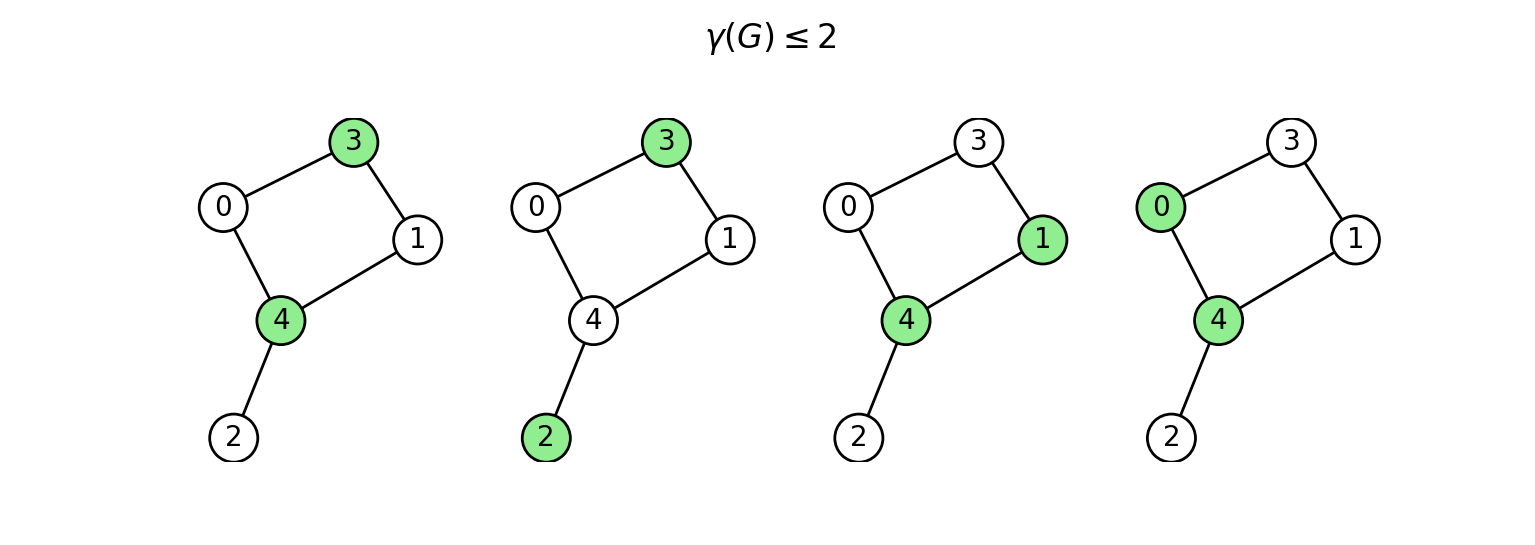
\includegraphics[width=0.64\textwidth]{mds-sol-n5-s.png}
	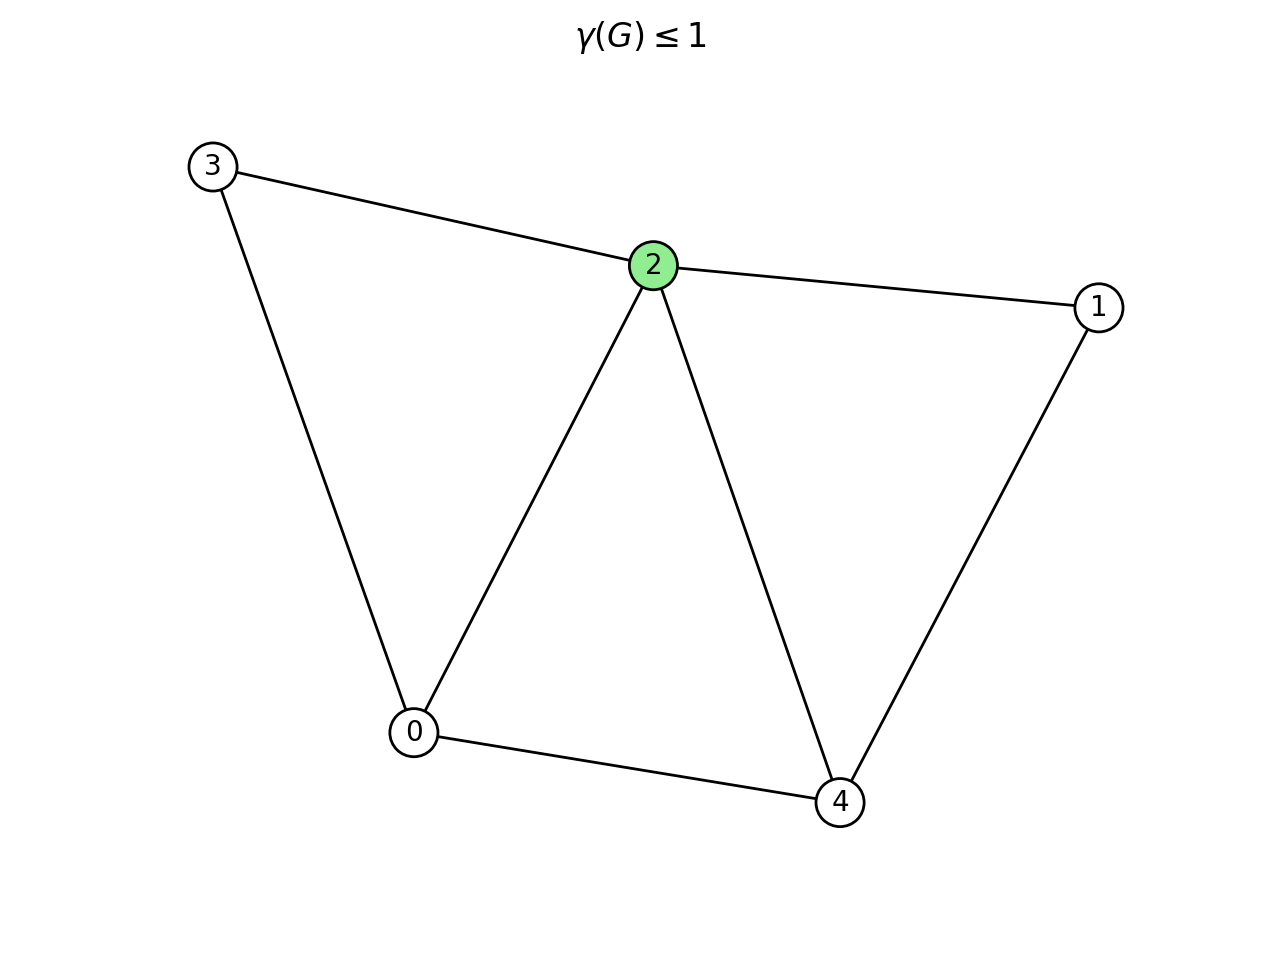
\includegraphics[width=0.32\textwidth]{mds-sol-n5.png}
	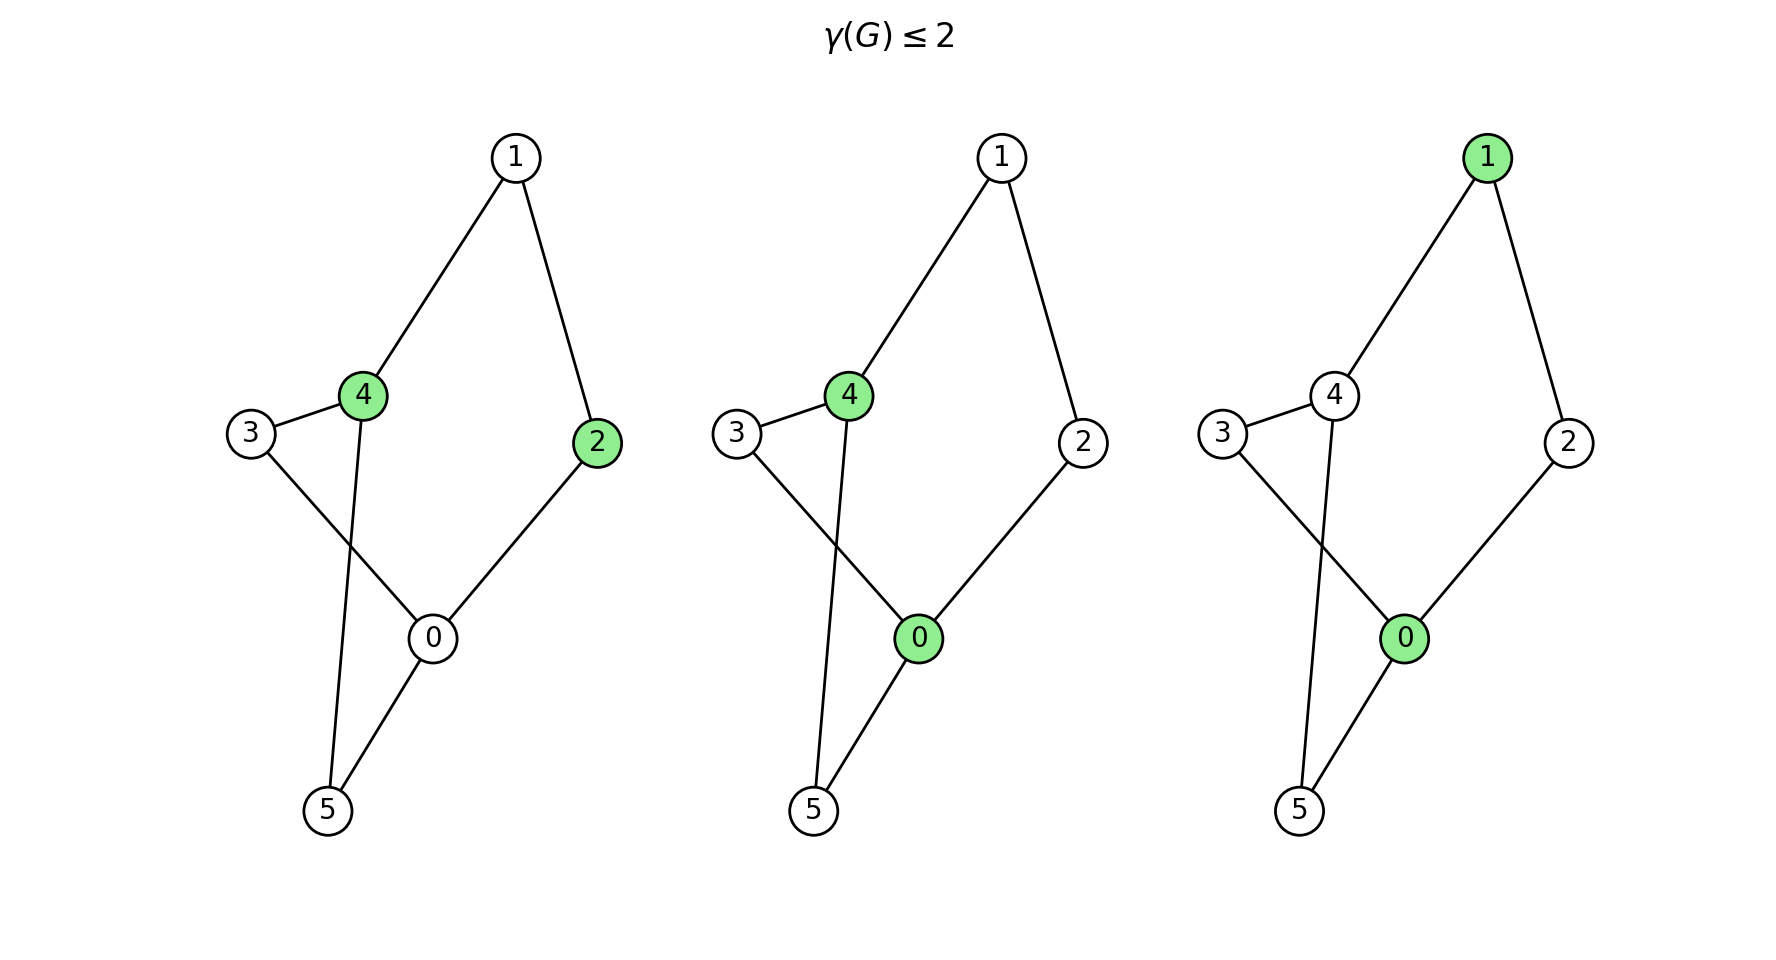
\includegraphics[width=0.49\textwidth]{mds-sol-n6.png}
	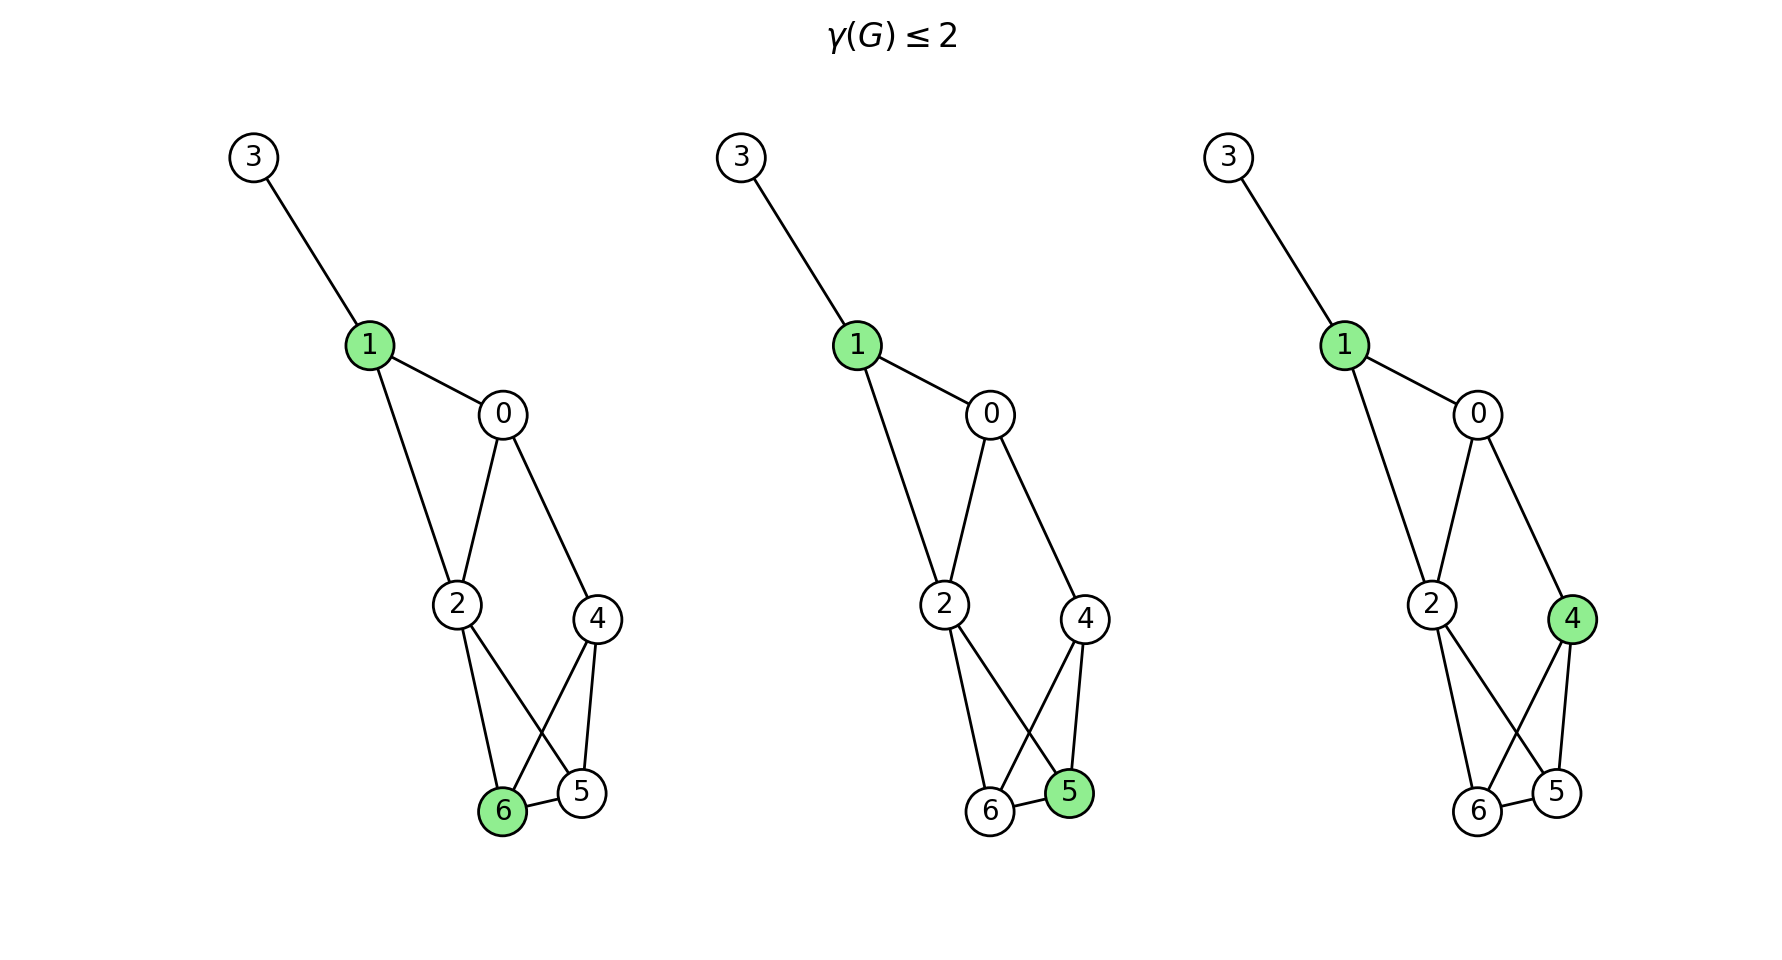
\includegraphics[width=0.49\textwidth]{mds-sol-n7.png}
	\caption{
		\label{fig:mds-sol-1} Vertex representation for global minimum solution of $\vec \psi \cdot Q \cdot \vec \psi$ for random 5-, 6- and 7-vertex graphs.
		Green vertices are included in the MDS.
	}
\end{figure}

\section{Ideas}
\subsection{Penalty as a function of annealing time}
The annealer encodes
\begin{equation}
	H(s) = (1-s)H_{init} + s H_{final} \, ,
\end{equation}
where $s$ is the annealing time.

If our final Hamiltonian is linear in a computation parameter time, then we can ramp up this parameter as a function of annealing time.

For example, in the MDS, we have
\begin{equation}
	H_{final} = H_{opt} + p H_{constraint} \, ,
\end{equation}
where $H_{opt} \leftrightarrow \sum_i x_i$ and $H_{constraint}$ encodes the Dominating set constraint.
To have $H_{final} = p \tilde{H}_{constraint}$, we have to place the optimization condition in $H_{constraint}$.

The idea here is: given a possible guess $\gamma$ for an MDS (which you can find using greedy search), is it possible to find a smaller solution.
In other words, you map $H_{opt}$ to a new constraint
\begin{equation}
	 H_{constraint} \mapsto  p  H_{constraint} + p  \tilde H_{opt} = p \tilde H_{final} 
	\, , \quad
	\tilde H_{opt} \leftrightarrow \sum_i x_i < \gamma \, .
\end{equation}
Note that in principle you can have different $p$s here.
You can now say that $p = \alpha s$ and ramp up the penalty as a function of annealing time.
Because you also get the wave function and now the energy (zero - const if constraints are fulfilled), you do also get a better solution if possible.
Also, since you ask for smaller, you might actually be lucky and get the optimal solution even if your guess was not really close.


\section{re-scale QUBO using ancillary qubits?}

Original qubo is
\begin{equation}
f= \psi^T Q \psi .
\end{equation}
We can re-scale Q by a factor of 2 like:
 \begin{align}
\psi_2 &= (\psi , \psi)^T \\
Q_2 &= 
\begin{pmatrix}
\frac{Q}{2} & 0 \\
0 & \frac{Q}{2} \\
\end{pmatrix} .
\end{align}
Then we have the re-scaled qubo:
\begin{align}
f &= \psi_2^T Q_2 \psi_2 \\
&=  \psi^T  \frac{Q}{2} \psi +  \psi^T  \frac{Q}{2} \psi \\
&=  \psi^T Q \psi .
\end{align}
The re-scaled qubo in general is
 \begin{align}
\psi_2 &= (\psi_a , \psi_b)^T \\
Q_2 &= 
\begin{pmatrix}
\frac{Q}{2} & 0 \\
0 & \frac{Q}{2} \\
\end{pmatrix} .
\end{align}
\begin{align}
f &= \psi_2^T Q_2 \psi_2 \\
&=  \psi_a^T  \frac{Q}{2} \psi_a +  \psi_b^T  \frac{Q}{2} \psi_b .
\end{align}
This function reaches the maximum if and only if both $\psi_a$ and $\psi_b$ are in the solution space.

\section{Asking MDS Question}
Instead of minimizing the size of the minimum dominating set under constraints, we can also ask if the number of nodes is smaller than an input dominating number
\begin{equation}
	\sum_{i \in V} x_i \leq \gamma_D \quad \Rightarrow \quad \sum_{i \in V} x_i - \gamma_D + s_D = 0 \, .
\end{equation}
This approach is interesting as it is constraints only.
Note that we still obtain solution vectors.
In principle this means one has to iterate approaches to get the best energy solution but it is also possible to find $E_0 = \gamma - n$ with $n\geq1$.
The QUBO now becomes
\begin{align}\label{mds2:qubo}
	Q &= 
	\begin{pmatrix}\alpha & \beta & 0 \\ 0 & \gamma & 0 \\ 0 & 0 & 0 \end{pmatrix}
	+
	A \begin{pmatrix}\alpha' & 0 & \beta' \\ 0 & 0 & 0 \\ 0 & 0 & \gamma' \end{pmatrix}
	\, , & 
	f(\vec x, \vec s, s_D)
	&=
	\vec \psi \cdot Q \cdot \vec \psi + |V| + A \gamma_D^2
	\, ,
\end{align}
where $\alpha, \beta, \gamma$ are the same as before and $\alpha', \beta', \gamma'$ implement the new constraint.
In particular 
\begin{align}
	\vec x \cdot \alpha' \vec x &= \left(\sum_i x_i\right)^2 - 2 \left(\sum_i x_i\right) \gamma_D 
	&& \Rightarrow &
	\alpha' &= \vec 1_x \vec 1_x^T - 2 \gamma_D \mathbbm{1}_x
	\\
	\vec x \cdot \beta' \vec s &= 2 \left(\sum_i x_i\right) s_D \gamma_D 
	&& \Rightarrow &
	\beta' &= 2 \gamma_D \vec 1_x B'
	\\
	\vec s \cdot \gamma' \vec s &= s_D^2 - 2 s_D \gamma_D 
	&& \Rightarrow &
	\alpha' &= B'^T B' - 2 \gamma_D B'
	\\
\end{align}


\section{Time-dependent simulation of quantum annealing}

I tried to follow DWave's convention as much as I can.
This notebook is to solve for time evolution dynamics of quantum annealing Hamiltonian. Then use final wavefunction to check the overlap with the Ising ground state from exact diagonalization. The absolute square of the overlap is the probability that the measurement result gives the solution. This is like what Nishimori did in his original paper.

Time dependent Hamiltoniain is
\begin{align}
\label{eq:annealH}
H_{anneal}(t) =  - \sum_i  A_i(t)\sigma^x_i +  \sum_{i>j} \sqrt{B_{i}(t)B_{j}(t)} J_{ij} \sigma^z_i \sigma^z_j +\sum_i B_{i}(t) h_i \sigma^z_i  ,
\end{align}
where $A_i(t)$ and $B_{i}(t)$ are site-dependent annealing schedule functions. The site-dependence taking into account of possible annealing offsets.

The goal is to solve the time-dependent Schrodinger equation 
\begin{align}
i \hbar \partial_t \psi(t) = H(t) \psi(t) .
\end{align}

The initial condition is the ground state of $H(s=0)$. This state is slightly different from the pure transverse  field eigenstate $\psi(t=0)= \otimes_i  |\rightarrow \rangle_i$, because the annealing schedule $B_i(s=0)> 0$.

The time period is set to $[0,1]$. 

The probability to get the ground state at measurement is
\begin{align}
P =\sum_{i\in G} | \langle \psi (t)  | \mbox{gnd}_i \rangle |^2 ,
\end{align}
where $\{ | \mbox{gnd}_i \rangle | i \in G \}$ forms an orthonormal basis, e.g. $\langle \mbox{gnd}_j | \mbox{gnd}_i \rangle = \delta_{ij}$,  for the degenerated ground states subspace.


\begin{figure}[htb]
	\centering
	%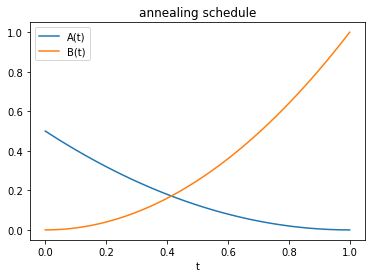
\includegraphics[width=0.5\textwidth]{annealingschedule.png}
	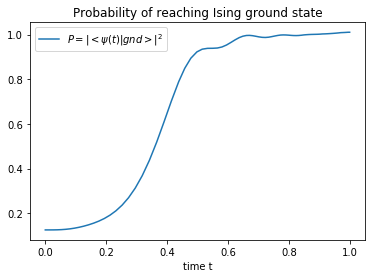
\includegraphics[width=0.5\textwidth]{probt.png}
	\caption{
		\label{tdse} time-dependent Schrodinger equation simulation of quantum annealing. Annealing time=100 $\mu s$.
	}
\end{figure}


For mixed state simulation the initial density matrix is the Gibbs canonical ensemble
\begin{equation}
\rho (0) =  \frac{e^{-\beta H(0)}}{\mbox{Tr}[e^{-\beta H(0)}]} .
\end{equation}
The time evolution of density matrix is governed by von Neumann equation
\begin{align}
i \hbar \partial_t \rho (t) = [H(t) , \rho(t)] ,
\end{align}
where $[,]$ denotes the Lie bracket.

The probability to get the ground state at measurement is
\begin{align}
P =  \mbox{Tr} \{  \rho (t) \pi_{\mbox{gnd}} \}  ,
\end{align}
where the projection operator onto the degenerated ground states subspace is $\pi_{\mbox{gnd}}=\sum_{i\in G} |\mbox{gnd}_i\rangle \langle \mbox{gnd}_i| $.


To include the decoherence effects, we solve for master equation in Lindblad form
\begin{align}
  \partial_t \rho (t) = - \frac{-i}{\hbar} [H(t) , \rho(t)] + \sum_j (2L_j \rho(t) L_j^\dagger - \{ L^\dagger_j L_j, \rho(t) \}) ,
\end{align}
where $L_j$ are the Lindblad operators for decoherence. In this study we only include lowest order approximation, i.e., the amplitude damping for non-interacting qubits. The Lindblad operator is $L_j=\sqrt{\gamma} \sigma^{+}_j$ for $h_j>0$ and $L_j=\sqrt{\gamma} \sigma^{-}_j$ for $h_j<0$, where $\gamma=1/T_1$ is the decoherence rate for relaxation time $T_1$. For simplicity we assume all qubits having the same relaxation time.




\subsection{unit conversion}

So this part is typed up just to fix units and $2\pi$ not for correct math, please check if this makes sense...


We have time $t \in [0,T]$ where $T=N_T \times 10^{-6} sec$ is annealing time with unit of micro sec. $N_T$ is just dimensionless number. The time is mapped to the dimensionless schedule $s\in [0,1]$ through $s=t/T$.

Now the equation we are solving is
\begin{equation}
 i \hbar \frac{d}{dt}\psi = H \psi .
\end{equation}

The dimension of the Hamiltonian is $[H]=N_H \times GHz \times h =N_H \times 10^9  \times h/( sec)$ where $N_H$ is the dimensionless numerical value. See 
\href{https://docs.dwavesys.com/docs/latest/c_qpu_0.html#quantum-annealing-with-ising-spins-in-a-transverse-field}{DWave documentation} Fig. 72. The Hamiltonian of Eq.~(\ref{eq:annealH}) only has units in $A(s)$ and $B(s)$ and are given by DWave as GHz, or $\mathrm{energy}/h$ and not $\hbar$.
Use
\begin{equation}
\frac{d}{dt}\psi = \frac{d}{Tds}\psi .
\end{equation}
So the equation is
\begin{align}
  \frac{d}{ds}\psi  &=  -i \frac{H\times T}{\hbar} \psi  &\\
   &=  -i \frac{N_H \times 10^9 \times h \times N_T \times 10^{-6} sec}{ sec  }\frac{2\pi}{h} \psi &  \\
  &= -i N_H \times N_T \times 10^{3} \times (2\pi) \psi  &.
\end{align}
and this is why the factor $10^{3} \times (2\pi)$.

\subsection{Simulating DWave}
To simulate DWave, we have to consider multiple systematic effects which cause deviation from exact solutions of the Schrödinger equation.
For example, interactions of the final Hamiltonian are present at the beginning of the anneal schedule due to non-zero anneal coefficients $B(s)$.
We expect a contamination of the ground state at the order of $B(0) \sim 5\%$ and allow to include these effects in our simulation by computing the ground state of the pure (only $H_\mathrm{init}$) or mixed (both $A(0) H_\mathrm{init} + B(0) H_\mathrm{final}$) system.
The Hamiltonian at the end of the anneal is less contaminated with $A(1) \sim 10^{-7}$.
In our simulation we also allow to define arbitrary annealing schedules as shown in Fig.~\ref{fig:anneal_schedules}.

Another systematic error is introduced when allowing different qubit-wise anneal schedules $A(s) \to A_i(s)$ and $B(s) \to B_i(s)$.
If $B_i(0) \neq B_j(0)$ for $i \neq j$ the initial Hamiltonian, and if $B_i(1) \neq B_j(1)$ for $i \neq j$ the final Hamiltonian is effectively different from what was implemented.
Therefore shifted anneal schedules on DWave cannot be set too large. We also allow our simulations to incorporate different qubit offsets as suggested by Eq.~(\ref{eq:annealH}), with an example annealing schedule shown in Fig.~\ref{fig:anneal_offset} as well.
It in principle possible to extend the anneal schedule beyond the range $s \in [s_I, s_F]$ with $s_I < 0$ and $s_F > 1$ such that, depending on how the $B_i$ are extrapolated, $B_i(s_I) = B_j(s_I)$ and $B_i(s_F) = B_j(s_F)$ for $i \neq j$ and equivalently for the $A_i$.
Therefore, we allow for extended anneal schedules, which allow all qubits to undergo the full annealing process, yielding a true temporal offset for inhomogeneous driving fields.

At the level of the scripts the problem that we solve are MDS for graph problems. In there, there is an option
\begin{itemize}
	\item \texttt{embed}: This embeds the QUBO into a chimera graph. Currently there is only an explicit result from G(2). I will in the future actually embed with DWave minorminer.
\end{itemize}

The options for controlling the annealing time and annealing schedule are:
\begin{itemize}
	\item \texttt{annealing\_time}: annealing time as defined from $s=[0, 1]$ in microseconds
	\item \texttt{normalized\_time}: this is $s$. Set it to $<0$ or $>1$ if offset is used to allow for a complete annealing schedule. The total time in microseconds will increase accordingly.
	\item \texttt{offset}: This is a string argument to the \texttt{fcn} method of the class \texttt{AnnealOffset} in \texttt{qlp.mds.mds\_qlpdb}. Define your own anneal offset routine here or call an existing one. E-mail me if you need more explanation.
	\item \texttt{fill\_value}: If \texttt{normalized\_time} is extended beyond (0, 1), this option decides whether to extrapolate the anneal schedule, or truncate it at the nearest value.
	\item \texttt{offset\_min}: Argument to \texttt{AnnealOffset} class.
	\item \texttt{offset\_range}: Argument to \texttt{AnnealOffset} class.
\end{itemize}

\begin{figure}[htb]
	\centering
	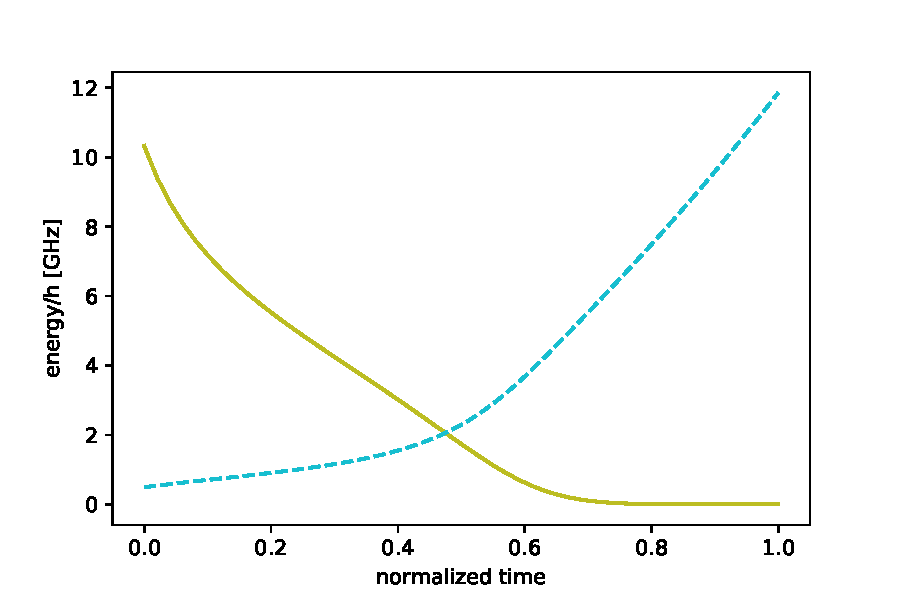
\includegraphics[width=0.49\textwidth]{coefficient_dwave.pdf}
	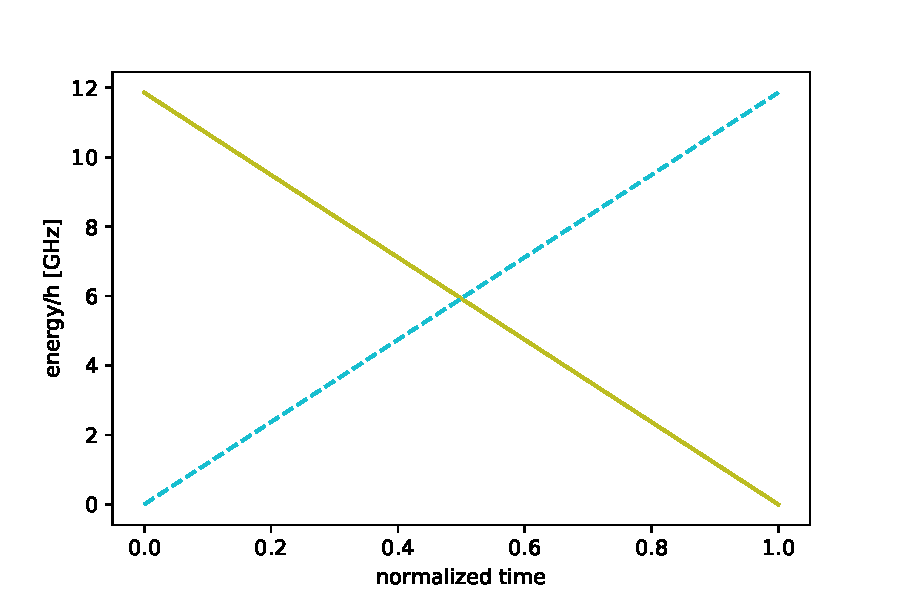
\includegraphics[width=0.49\textwidth]{coefficient_linear.pdf}
	\caption{\label{fig:anneal_schedules} Examples of anneal schedules. In figure are value of $A(s)$ and $B(s)$ as a function of normalized time $s$. The DWave schedule (left), and a idealized linear annealing schedule (right).
	}
\end{figure}

\begin{figure}[htb]
	\centering
	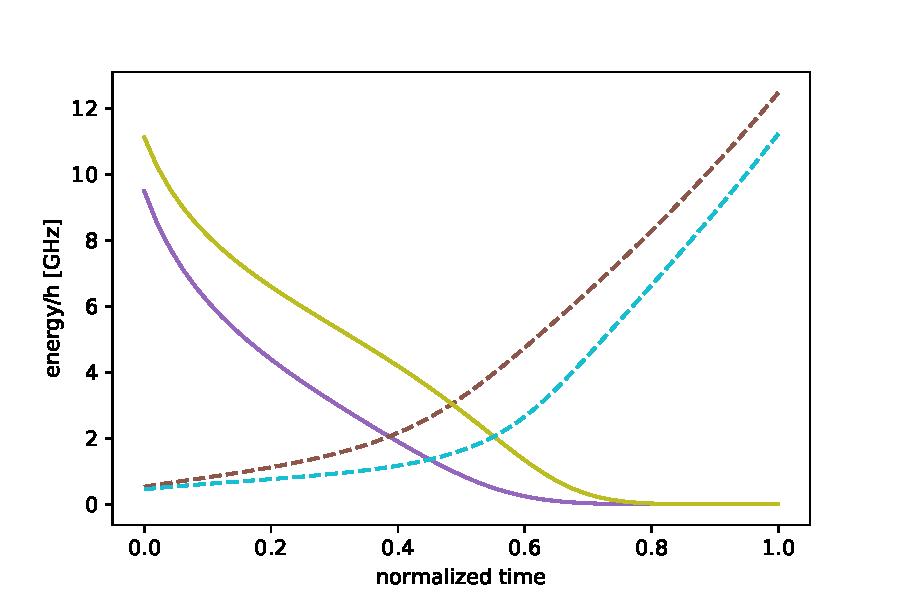
\includegraphics[width=0.49\textwidth]{coefficient_dwave_offset.pdf}
	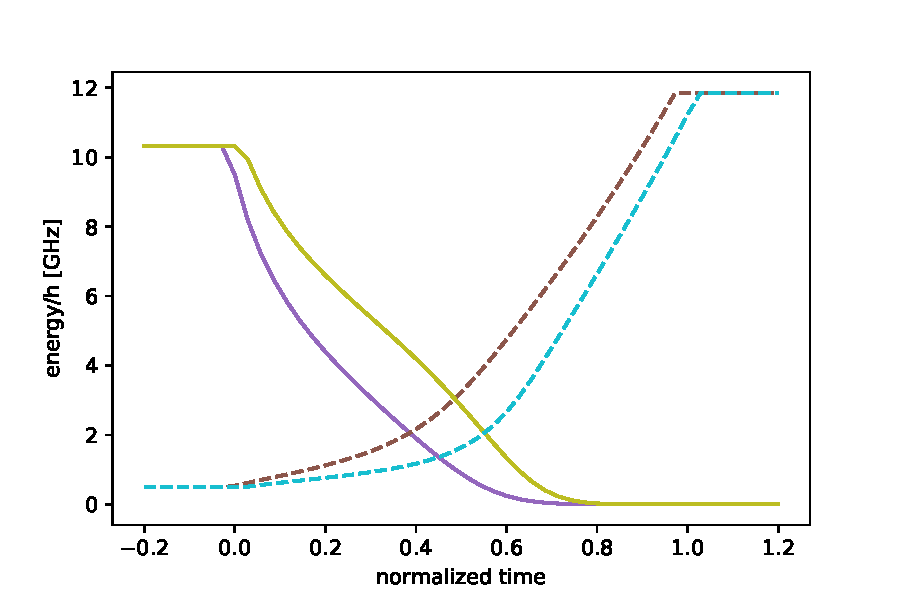
\includegraphics[width=0.49\textwidth]{coefficient_dwave_offset_full.pdf}
	\caption{\label{fig:anneal_offset} (left) Dwave schedule with offset. Note that the values of $A(s)$ and $B(s)$ are no longer the same for all qubits at the start and end of the anneal. (right) An extended anneal schedule that allows all qubits to start and end with the same coefficients.
	}
\end{figure}

The ODE solver we currently call is from \texttt{scipy.integrate.solve\_ivp}. In the future, we should consider migrating this to use \texttt{qutip.ssesolve} or some equivalent. See \href{http://qutip.org/docs/latest/guide/dynamics/dynamics-time.html}{QuTiP time-dependent solvers Documentation}. For now, the solver parameters are
\begin{itemize}
	\item \texttt{method}: The default is RK45, which is a 5th order Runge-Kutta algorithm.
	\item \texttt{rtol}: The relative tolerance for the solver.
	\item \texttt{atol}: The absolute tolerance.
\end{itemize}

We have also implemented both a pure-state simulation, as well as a mixed-state simulation.
These can be chosen with the following parameters:

\begin{itemize}
	\item \texttt{pure\_tdse}: This is a boolean (True / False) flag and runs the pure state solver.
	\item \texttt{mixed\_tdse}: This boolean flag runs the mixed state solver.
	\item \texttt{temp}: This sets the temperature for the mixed state solver in kelvins.
	\item \texttt{initial\_wavefunction}: For the pure state solver, the initial wavefunction can be chosen to be the ground state of $\sum_i \sigma_i^x$ (\texttt{transverse}) or $H(0)$ (\texttt{real}). For the DWave anneal schedule, or when annealing offsets are used without extended annealing times, these two options are not the same.
	\item \texttt{degeneracy\_tol}: This sets the numerical tolerance as to when an excited-state is labeled as degenerate to the ground state. This is important for graphs with degenerate ground states.
\end{itemize}

A quick study below. We run a simulation with anneal offsets similar to what we ran on DWave (Fig.~\ref{fig:dwave_result}). We see that if we apply a delay on qubits with small values and advance qubits with of $h_i$ (binary), then the performance improves. And vice versa. This is completely unexpected from the point of view of many-body localization. Because this result was so surprising, we wrote this simulator. Under DWave conditions (embedded problem, non-linear anneal schedule, truncating offset), we are able to reproduce this behavior (fig~\ref{fig:proba_dwave}). Here I note that if we run the idealized scenario (more importantly, without embedding), the behavior is reverse, and is consistent with what is expected due to many-body localization.

\begin{figure}[htb]
	\centering
	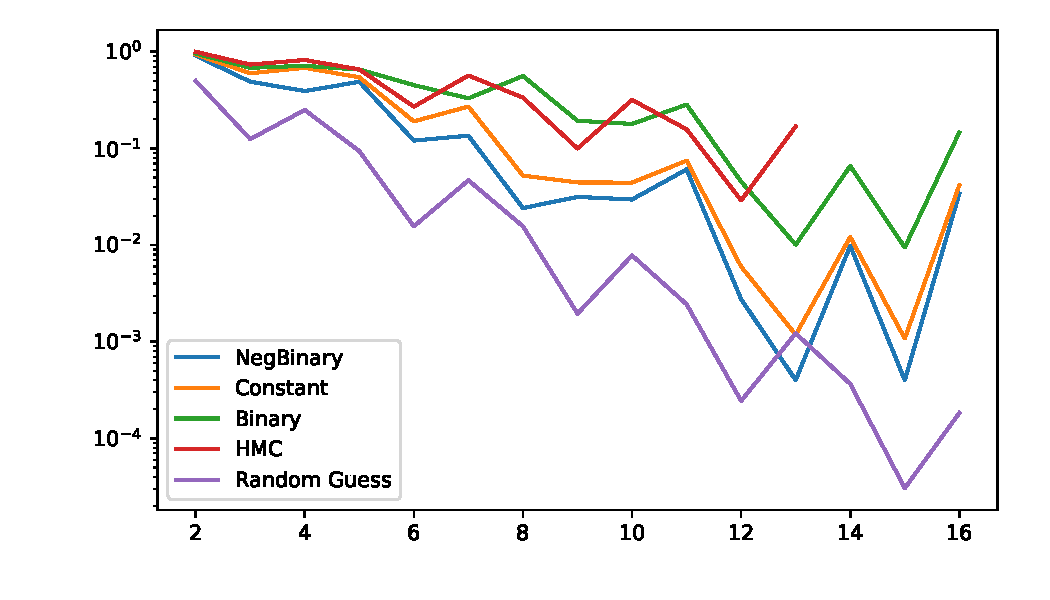
\includegraphics[width=0.8\textwidth]{scaling_full_0p10.pdf}
	\caption{\label{fig:dwave_result} DWave results.
	}
\end{figure}


\begin{figure}[htb]
	\centering
	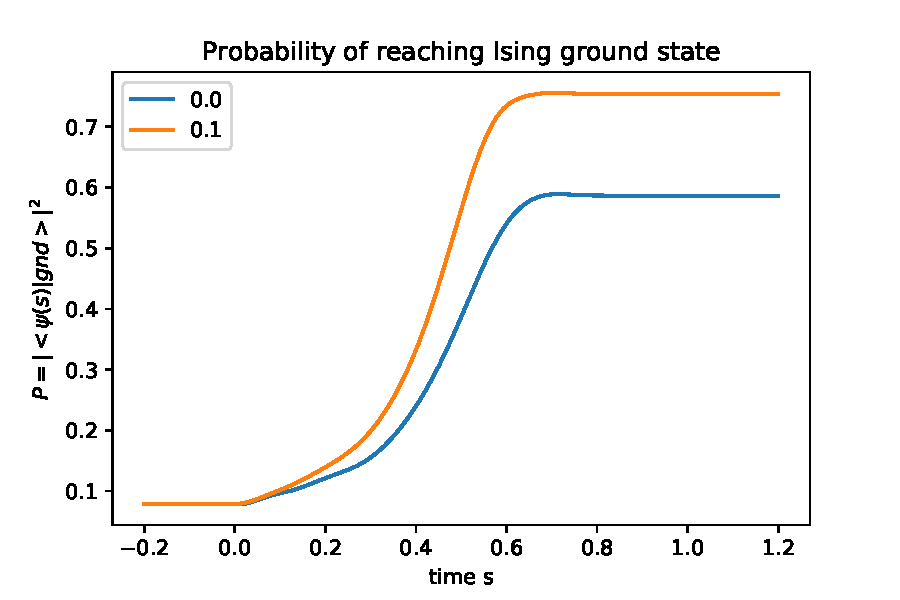
\includegraphics[width=0.49\textwidth]{proba_binary.pdf}
	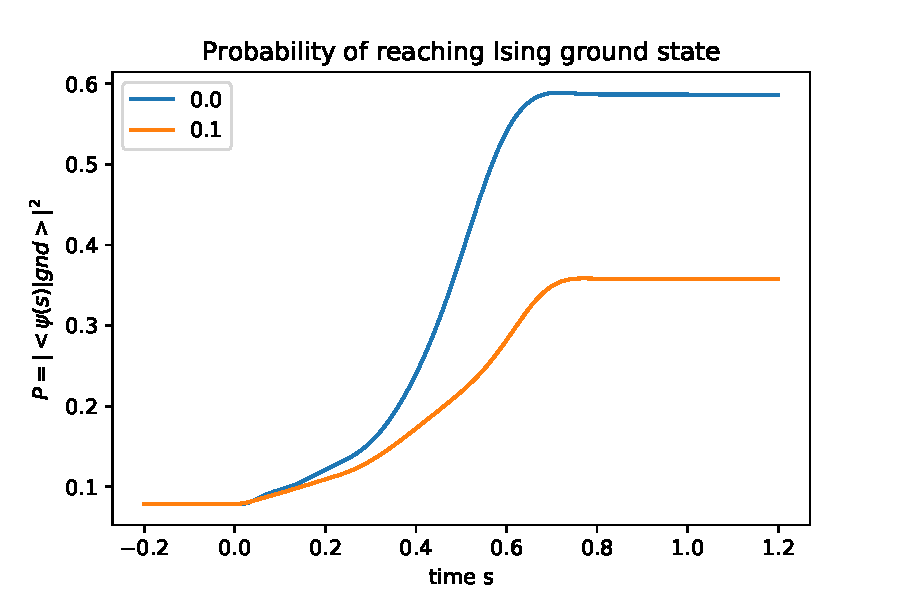
\includegraphics[width=0.49\textwidth]{proba_negbinary.pdf}
	\caption{\label{fig:proba_dwave} (left) Binary offset and (right) NegBinary offset.
	}
\end{figure}

\end{document}
